\section{Definicja anomalii (obserwacji odstającej)}
Obserwacje odstające to punkty, które nie odpowiadają wzorcowi w zbiorze danych. Barnett i Lewis definiują obserwację odstającą następująco: ,,Obserwacja odstająca jest to obserwacja, której obecność jest różna od pozostałych obserwacji'' \cite{barnett1984outliers}. Rysunek \ref{fig:anomalia} obrazuje przykład obserwacji odstających (anomalii) dla dwuwymiarowego zbioru danych. Zbiór danych posiada obszar wzorcowy {$N_1$}, większość punktów leży wewnątrz tego obszaru. Punkty wystarczająco oddalone od obszaru $N_1$: $o_1$, $o_2$, $o_3$ -- sklasyfikowane są jako obserwacje odstające (anomalie).
\begin{figure}
    \centering
    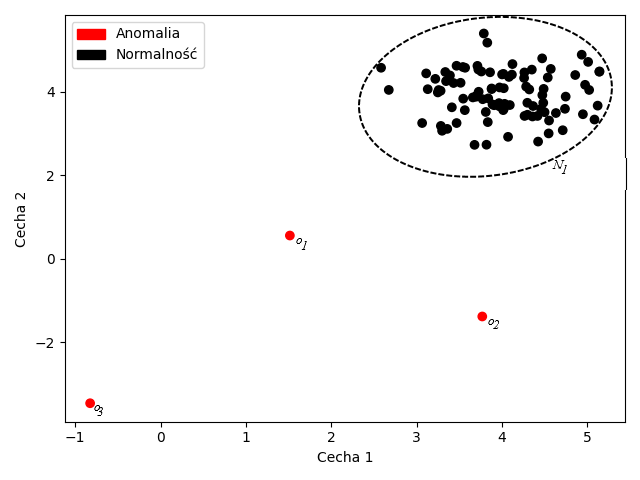
\includegraphics[width=.5\textwidth]{chapters/istniejace/images/anomalia.png}
    \caption{Prosty przykład anomalii w dwuwymiarowym zbiorze danych}
    \label{fig:anomalia}
\end{figure}

\section{Zadanie detekcji anomalii}
W pracy rozważamy uczenie nienadzorowane na zbiorze $N$ punktów $x_1,...,x_N$ każdy punkt jest d-wymiarowym wektorem liczb rzeczywistych. Zbiór danych składa się z obserwacji poprawnych i anomalnych, jednakże zbiór nie posiada wektora $y_1,..,y_N$ -- klasyfikującego obserwację do obserwacji poprawnych lub anomalnych. Zadaniem jest identyfikacja punktów anomalnych w danym zbiorze. Zadanie detekcji anomalii jest zadaniem klasyfikacji jednoklasowej. 

\section{Różnice w podejściu detekcji anomalii}

\subsection{Wykrywanie anomalii lokalnych a globalnych}
Podejście dotyczy wyboru zakresu zbioru jako zbioru odniesienia dla rozpatrywania odstawania danej obserwacji. Głowne podejścia to: podejście globalne (Rysunek \ref{fig:global}) oraz lokalne (Rysunek\ref{fig:local}).
\begin{itemize}
    \item Podejście globalne 
    \begin{itemize}
        \item Zbiór danych obejmuje wszystkie obserwacje
        \item Założenie o istnieniu jeden prawidłowego mechanizmu generującego normalne punkty.
        \item Problem: inne obserwacje odstające mogą również występować w zbiorze danych zaburzając rezultat detekcji.
    \end{itemize}
    \item Podejście lokalne 
    \begin{itemize}
        \item Zbiór referencyjny jest podzbiorem całego zbioru
        \item Brak założenia o liczbie mechanizmów generujących.
        \item Problem: wybór odpowiedniego podzbioru
    \end{itemize}
\end{itemize}

\begin{figure}[]
  \centering
  \begin{minipage}{0.4\textwidth}
    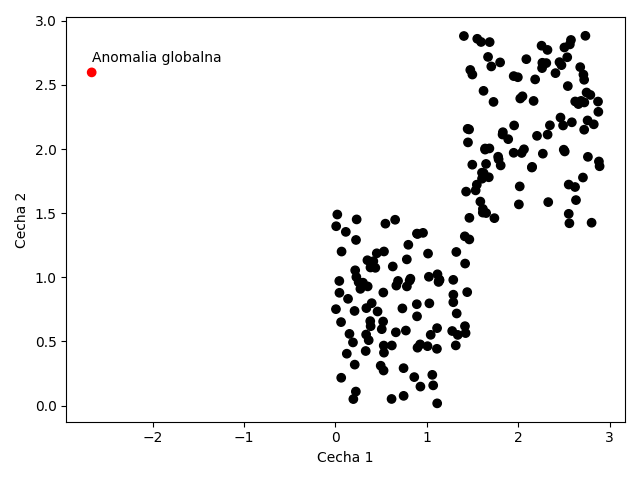
\includegraphics[width=\textwidth]{chapters/istniejace/images/anomalia_globalna.png}
    \caption{Przykład anomalii globalnej}
    \label{fig:global}
  \end{minipage}
  \hfill
  \begin{minipage}{0.4\textwidth}
    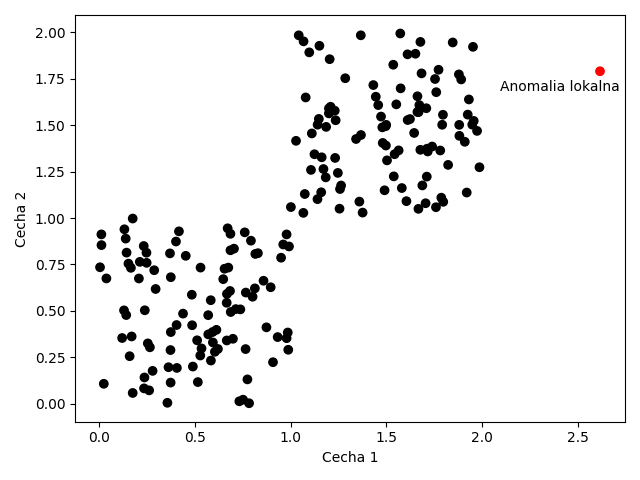
\includegraphics[width=\textwidth]{chapters/istniejace/images/anomalia_lokalna.png}
    \caption{Przykład anomalii lokalnej }
    % A comperative evaluation ma lepszy obraz
    \label{fig:local}
  \end{minipage}
\end{figure}

\subsection{Wynik metody}
Ważnym aspektem dla metody wykrywania anomalii jest sposób oceny każdej obserwacji. Dane wyjściowe metody mogą przypisywać obserwacji wartość anomalności na dwa warianty:
\begin{itemize}
    \item binarny: przypisanie obserwacji etykiety normalnej obserwacji lub anomalnej
    \item ciągły: dla każdej obserwacji obliczany jest wynik anomalności np. prawdopodobieństwo obserwacji jako anomalii
\end{itemize}
Wiele podejść opartych na przypisywaniu wyniku anomalności skupia się na wyznaczeniu grupy n-obserwacji o najwyższym wyniku (parametr n często podawany jest przez użytkownika np. wartość kontaminacji). Również z tego podejścia można za pomocą np. progu wyniku anomalności otrzymać binarną etykietę obserwacji dzięki temu osoba analizująca dane może dostosować próg dla danej dziedziny.

\subsection{Podejścia w konstrukcja metody detekcji anomalii} 
\begin{itemize}
    \item Parametryczna
    \item Nieparametryczna
\end{itemize}
Przykład technik opisany szerzej w sekcji \ref{section:methods}

\section{Przykłady technik wykrywania anomalii}
\label{section:methods}

\subsection{Podejście statystyczne}
Pierwsze badania anomalii oraz metod ich wykrywania polegały na modelowaniu statystycznym. Anomalie mogą zaburzać zadania: estymacji, predykcji czy klasyfikacji. Pojawienie się anomalii powoduje zmianę m.in. średniej z próby i wariancje. 


\section{Problematyka}

\section{Porównanie metod}
Ewaluacja algorytmów dla problemu wykrywania anomalii jest problematyczna. Brak powszechnie dostępnej bazy zbiorów danych czy uniwersalnej metody oceny działania wymusił 